% questions.tex —— 1988 年·全国卷·理科 · 题目内容片段（无答案）
% 由 tools/generate_projects.py 依来源总账自 1988/1988_数学真题_全国理_试题.md 生成，勿手改（改源 MD 后重跑）


\gkpart{理科数学}

\begin{gktip}
\textbf{来源说明}：本题面依据固定源 PDF《1988 普通高等学校招生考试（全国卷理）》逐题转录。固定源共 1 页、原卷印刷页码 32；PDF 含题面文字层和矢量图形，但不含答案、解析或评分标准，以下答案和解析由本库独立推导。

\textbf{图形说明}：第 9、19、22 题的正四棱台、四棱锥和正三棱锥图依据固定源图形关系重绘为 TikZ 矢量图。
\end{gktip}

\begin{question}
\gkti{1}复数

\nopagebreak[4]
\[
\left(\frac{1-i}{1+i}\right)^2
\]

的值等于\mbox{（　　）}

（A）$1$　　（B）$-1$　　（C）$i$　　（D）$-i$

\end{question}
\begin{question}
\gkti{2}设圆 $M$ 的方程为

\nopagebreak[4]
\[
(x-3)^2+(y-2)^2=2,
\]

\Needspace{5\baselineskip}
直线 $L$ 的方程为

\nopagebreak[4]
\[
x+y-3=0,
\]

点 $P$ 的坐标为 $(2,1)$，那么\mbox{（　　）}

（A）点 $P$ 在直线 $L$ 上，但不在圆 $M$ 上

（B）点 $P$ 在圆 $M$ 上，但不在直线 $L$ 上

（C）点 $P$ 既在圆 $M$ 上，又在直线 $L$ 上

（D）点 $P$ 既不在直线 $L$ 上，也不在圆 $M$ 上

\end{question}
\begin{question}
\gkti{3}集合 $\{1,2,3\}$ 的子集共有\mbox{（　　）}

（A）7 个　　（B）8 个　　（C）6 个　　（D）5 个

\end{question}
\begin{question}
\gkti{4}已知双曲线方程

\nopagebreak[4]
\[
\frac{x^2}{20}-\frac{y^2}{5}=1,
\]

那么它的焦距是\mbox{（　　）}

（A）$10$　　（B）$5$　　（C）$\sqrt{15}$　　（D）$2\sqrt{15}$

\end{question}
\begin{question}
\gkti{5}在

\nopagebreak[4]
\[
(x-\sqrt3)^{10}
\]

的展开式中，$x^6$ 的系数是\mbox{（　　）}

（A）$-27C_{10}^{6}$　　（B）$27C_{10}^{4}$

（C）$-9C_{10}^{6}$　　（D）$9C_{10}^{4}$

\end{question}
\begin{question}
\gkti{6}函数

\nopagebreak[4]
\[
y=\cos^4x-\sin^4x
\]

的最小正周期是\mbox{（　　）}

（A）$\pi$　　（B）$2\pi$　　（C）$\dfrac\pi2$　　（D）$4\pi$

\end{question}
\begin{question}
\gkti{7}方程

\nopagebreak[4]
\[
4\cos^2x-4\sqrt3\cos x+3=0
\]

的解集是\mbox{（　　）}

（A）$\left\{x\mid x=k\pi+(-1)^k\frac\pi6,\ k\in\mathbb Z\right\}$

（B）$\left\{x\mid x=k\pi+(-1)^k\frac\pi3,\ k\in\mathbb Z\right\}$

（C）$\left\{x\mid x=2k\pi\pm\frac\pi6,\ k\in\mathbb Z\right\}$

（D）$\left\{x\mid x=2k\pi\pm\frac\pi3,\ k\in\mathbb Z\right\}$

\end{question}
\begin{question}
\gkti{8}极坐标方程

\nopagebreak[4]
\[
\rho=\frac4{3-2\cos\theta}
\]

所表示的曲线是\mbox{（　　）}

（A）圆　　（B）双曲线右支　　（C）抛物线　　（D）椭圆

\Needspace{0.4\textheight}
\end{question}
\begin{question}
\gkti{9}如图，正四棱台中，$A'D'$ 所在的直线与 $BB'$ 所在的直线是\mbox{（　　）}
\nopagebreak[4]
\begin{center}% 1988 年全国卷理科第 9 题：正四棱台
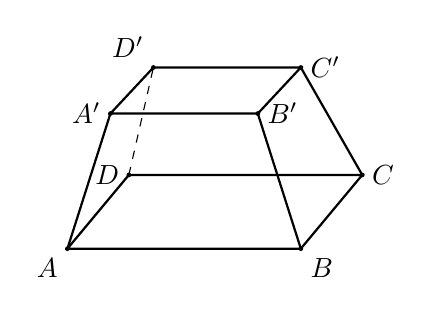
\begin{tikzpicture}[scale=0.78,>=stealth]
  \coordinate (A) at (0,0);
  \coordinate (B) at (3.8,0);
  \coordinate (C) at (4.8,1.2);
  \coordinate (D) at (1.0,1.2);
  \coordinate (Ap) at (0.7,2.2);
  \coordinate (Bp) at (3.1,2.2);
  \coordinate (Cp) at (3.8,2.95);
  \coordinate (Dp) at (1.4,2.95);
  \draw[thick] (A)--(B)--(C)--(D)--cycle;
  \draw[thick] (Ap)--(Bp)--(Cp)--(Dp)--cycle;
  \draw[thick] (A)--(Ap) (B)--(Bp) (C)--(Cp);
  \draw[dashed] (D)--(Dp);
  \fill (A) circle (1.1pt) node[below left] {$A$};
  \fill (B) circle (1.1pt) node[below right] {$B$};
  \fill (C) circle (1.1pt) node[right] {$C$};
  \fill (D) circle (1.1pt) node[left] {$D$};
  \fill (Ap) circle (1.1pt) node[left] {$A'$};
  \fill (Bp) circle (1.1pt) node[right] {$B'$};
  \fill (Cp) circle (1.1pt) node[right] {$C'$};
  \fill (Dp) circle (1.1pt) node[above left] {$D'$};
\end{tikzpicture}
\end{center}
\nopagebreak[4]
（A）相交直线　　（B）平行直线

（C）不互相垂直的异面直线　　（D）互相垂直的异面直线

\end{question}
\begin{question}
\gkti{10}

\nopagebreak[4]
\[
\tan\left(\arctan\frac15+\arctan3\right)
\]

的值等于\mbox{（　　）}

（A）$4$　　（B）$\dfrac12$　　（C）$\dfrac18$　　（D）$8$

\end{question}
\begin{question}
\gkti{11}设命题甲：$\triangle ABC$ 的一个内角为 $60^\circ$；命题乙：$\triangle ABC$ 的三内角的度数成等差数列。那么\mbox{（　　）}

（A）甲是乙的充分条件，但不是必要条件

（B）甲是乙的必要条件，但不是充分条件

（C）甲是乙的充要条件

（D）甲不是乙的充分条件，也不是乙的必要条件

\end{question}
\begin{question}
\gkti{12}在复平面内，若复数 $z$ 满足

\nopagebreak[4]
\[
|z+1|=|z-i|,
\]

则 $z$ 所对应的点 $Z$ 的集合构成的图形是\mbox{（　　）}

（A）圆　　（B）直线　　（C）椭圆　　（D）双曲线

\end{question}
\begin{question}
\gkti{13}如果曲线

\nopagebreak[4]
\[
x^2-y^2-2x-2y-1=0
\]

\Needspace{5\baselineskip}
经过平移坐标轴后的新方程为

\nopagebreak[4]
\[
x'^2-y'^2=1,
\]

那么新坐标系的原点在原坐标系中的坐标为\mbox{（　　）}

（A）$(1,1)$　　（B）$(-1,-1)$　　（C）$(-1,1)$　　（D）$(1,-1)$

\end{question}
\begin{question}
\gkti{14}假设在 200 件产品中有 3 件次品，现在从中任意抽取 5 件，其中至少有 2 件次品的抽法有\mbox{（　　）}

（A）$C_3^2C_{197}^3$ 种

（B）$C_3^2C_{197}^3+C_3^3C_{197}^2$ 种

（C）$C_{200}^5-C_{197}^5$ 种

（D）$C_{200}^5-C_3^1C_{197}^4$ 种

\end{question}
\begin{question}
\gkti{15}已知二面角 $\alpha-AB-\beta$ 的平面角是锐角，$C$ 是平面 $\alpha$ 内一点（它不在棱 $AB$ 上），点 $D$ 是点 $C$ 在面 $\beta$ 上的投影，点 $E$ 是棱 $AB$ 上满足 $\angle CEB$ 为锐角的任一点，那么\mbox{（　　）}

（A）$\angle CEB>\angle DEB$

（B）$\angle CEB=\angle DEB$

（C）$\angle CEB<\angle DEB$

（D）$\angle CEB$ 与 $\angle DEB$ 的大小关系不能确定

\end{question}
\begin{question}
\gkti{16}求复数

\nopagebreak[4]
\[
\sqrt3-i
\]

的模和辐角的主值。

\end{question}
\begin{question}
\gkti{17}解方程

\nopagebreak[4]
\[
9^{-x}-2\cdot3^{1-x}=27.
\]

\end{question}
\begin{question}
\gkti{18}已知

\nopagebreak[4]
\[
\sin\theta=-\frac35,\qquad
3\pi<\theta<\frac{7\pi}{2},
\]

\Needspace{5\baselineskip}
求

\nopagebreak[4]
\[
\tan\frac\theta2.
\]

\Needspace{0.4\textheight}
\end{question}
\begin{question}
\gkti{19}如图，四棱锥 $S-ABCD$ 的底面是边长为 $1$ 的正方形，侧棱 $SB$ 垂直于底面，并且

\nopagebreak[4]
\[
SB=\sqrt3.
\]

用 $\alpha$ 表示 $\angle ASD$，求 $\sin\alpha$。
\nopagebreak[4]
\begin{center}% 1988 年全国卷理科第 19 题：四棱锥
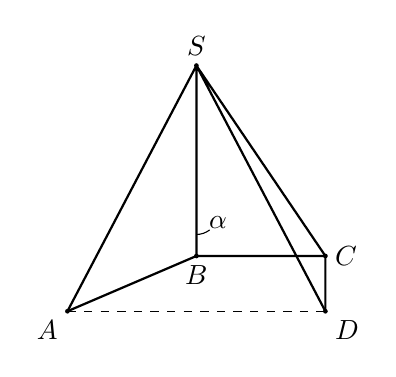
\begin{tikzpicture}[scale=0.78,>=stealth]
  \coordinate (S) at (2.1,4.0);
  \coordinate (B) at (2.1,0.9);
  \coordinate (A) at (0,0);
  \coordinate (C) at (4.2,0.9);
  \coordinate (D) at (4.2,0);
  \draw[thick] (S)--(A) (S)--(B) (S)--(C) (S)--(D);
  \draw[thick] (A)--(B)--(C)--(D);
  \draw[dashed] (A)--(D) (S)--(B);
  \draw (2.1,1.25) arc (-90:-52:0.35);
  \node at (2.45,1.45) {$\alpha$};
  \fill (S) circle (1.1pt) node[above] {$S$};
  \fill (A) circle (1.1pt) node[below left] {$A$};
  \fill (B) circle (1.1pt) node[below] {$B$};
  \fill (C) circle (1.1pt) node[right] {$C$};
  \fill (D) circle (1.1pt) node[below right] {$D$};
\end{tikzpicture}
\end{center}
\nopagebreak[4]
\end{question}
\begin{question}
\gkti{20}已知等比数列 $\{a_n\}$ 的公比 $q>1$，并且 $a_1=b$（$b\ne0$）。求

\nopagebreak[4]
\[
\lim_{n\to\infty}
\frac{a_1+a_2+a_3+\cdots+a_n}
{a_6+a_7+a_8+\cdots+a_n}.
\]

\end{question}
\begin{question}
\gkti{21}已知 $\tan x=a$，求

\nopagebreak[4]
\[
\frac{3\sin x+\sin3x}{3\cos x+\cos3x}
\]

的值。

\Needspace{0.4\textheight}
\end{question}
\begin{question}
\gkti{22}如图，正三棱锥 $S-ABC$ 的侧面是边长为 $a$ 的正三角形，$D$ 是 $SA$ 的中点，$E$ 是 $BC$ 的中点，求 $\triangle SDE$ 绕直线 $SE$ 旋转一周所得的旋转体的体积。
\nopagebreak[4]
\begin{center}% 1988 年全国卷理科第 22 题：正三棱锥及中点
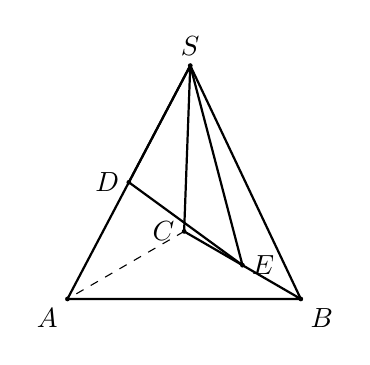
\begin{tikzpicture}[scale=0.78,>=stealth]
  \coordinate (S) at (2.0,3.8);
  \coordinate (A) at (0,0);
  \coordinate (B) at (3.8,0);
  \coordinate (C) at (1.9,1.1);
  \coordinate (D) at (1.0,1.9);
  \coordinate (E) at (2.85,0.55);
  \draw[thick] (S)--(A) (S)--(B) (S)--(C);
  \draw[thick] (A)--(B) (B)--(C);
  \draw[dashed] (C)--(A);
  \draw[thick] (S)--(E) (D)--(E) (S)--(D);
  \fill (S) circle (1.1pt) node[above] {$S$};
  \fill (A) circle (1.1pt) node[below left] {$A$};
  \fill (B) circle (1.1pt) node[below right] {$B$};
  \fill (C) circle (1.1pt) node[left] {$C$};
  \fill (D) circle (1.1pt) node[left] {$D$};
  \fill (E) circle (1.1pt) node[right] {$E$};
\end{tikzpicture}
\end{center}
\nopagebreak[4]
\end{question}
\begin{question}
\gkti{23}设 $a>0$，$a\ne1$，$t>0$，比较

\nopagebreak[4]
\[
\frac12\log_a t
\qquad\text{\text{与}}\qquad
\log_a\frac{t+1}{2}
\]

的大小，并证明你的结论。

\end{question}
\begin{question}
\gkti{24}给定实数 $a$，且 $a\ne0,\ a\ne1$，设函数

\nopagebreak[4]
\[
y=\frac{x-1}{ax-1}
\qquad\left(x\in R,\ x\ne\frac1a\right).
\]

证明：

（1） 经过这个函数图象上任意两个不同的点的直线不平行于 $x$ 轴；

（2） 这个函数的图象关于直线 $y=x$ 成轴对称图形。

\end{question}
\begin{question}
\gkti{25}直线 $L$ 的方程为

\nopagebreak[4]
\[
x=-\frac p2,\qquad p>0;
\]

\Needspace{5\baselineskip}
椭圆的中心为

\nopagebreak[4]
\[
D\left(2+\frac p2,0\right),
\]

\Needspace{5\baselineskip}
焦点在 $x$ 轴上，长半轴长为 $2$，短半轴长为 $1$，它的一个顶点为

\nopagebreak[4]
\[
A\left(\frac p2,0\right).
\]

问 $p$ 在哪个范围内取值时，椭圆上有四个不同的点，它们中每一个点到点 $A$ 的距离等于该点到直线 $L$ 的距离。

\end{question}